% !TXS template
\documentclass[12pt]{memoir}
\usepackage[T1]{fontenc}
\usepackage[utf8]{inputenc}
\usepackage{lmodern}
\usepackage[a4paper]{geometry}
\usepackage{graphics}
\usepackage{graphicx}
\usepackage{listings}
\usepackage{float}
\usepackage{hyperref}
\usepackage{multicol}
\setcounter{tocdepth}{3}
\setcounter{secnumdepth}{3}
\usepackage[font={small,it}]{caption}
\usepackage{subcaption}
%%\usepackage[margin=1.4in]{geometry}
%%\usepackage{babel}

%\addto\captionsfrench{% Replace "english" with the language you use
%	\renewcommand{\contentsname}%
%	{}%
%}
\renewcommand{\printtoctitle}[1]{\Huge \textbf{Table of Contents}}

\renewcommand\thefigure{\arabic{figure}}
\renewcommand\thetable{\arabic{table}}
\setcounter{figure}{0}
\renewcommand{\thesection}{\arabic{section}}
\begin{document}

\title{Apprenticeship thesis, 2nd years \\ \textbf{Master of Computer Science}, speciality \textbf{Ingénierie du
		Logiciel et des Connaissances} 
	
	\bigskip
	{\huge Realtime continous optimisation of healthcare transportation fleet using massively parallel memetic algorithm on GPGPU} \\	
	}
\author{Joseph Pallamidessi\\ University of Strasbourg} 
\date{\vspace{2.5in}
	
\protect\raggedright
{\normalsize Maître d'alternance:} \\
		\textbf{Pierre Collet}, Université de Strasbourg \\
		\textbf{Guillaume Philips}, Synovo SAS}

\maketitle
\newpage

\tableofcontents*
\newpage


\section{Acknowlegments}\label{Acknowledgements}

I would first like to thank professor Collet, for the guidance provided during those
two year of apprenticeship. It is because of him that today I stand before you,
having opened to me the wonderful world of universitary research. \\
Guillaume Philip, my apprenticeship tutor inside Synovo to having me let experiment, test
and gave full liberty to conduit my research on this problem during the one and a
half year that I spent inside his company. He was always listening, thoughtful and
focus even when the obstacle seemed unreachable. His flexibility, availability
and focus are something that I wish to encounter again in my carrier, as it gave me
the strength to finish this big challenge. \\
Jeremy Wies for my current position of research assistant at Synovo.
Thibault Thomas for his always optimistic mood and the overall help, on too many things to enumerate here. It was always a pleasure to discuss with him and I formally apologize for having him be my rubber duck while being stuck on problems. As a true believer of the concept serendipity, many aspect of the current work may have been indirectly influenced by our discussions. \\
Anne Juventy for having be a great help at a time the future of the project seemed
dire. It is by her ingenuity and practical mind that we were able to canalise our
thoughts.\\
Benjamin Chetioui for having be an efficient and resourceful coworker and his numerous inputs in all aspects of this project.


\bigskip
I would like to thanks the pedagogic team of the ILC Master and more specifically M. Narboux, M. Magaud, Mme. Mark-Zwecker for allowing me to have this unorthodox journey through theirs formation, even if it had add a lot of supplementary work on them. \\
I would like to thanks Synovo and the ICube laboratories for their support and
letting me work in this big collaboration between university researchers and the
corporate world.
Thanks to all my proofreaders and friends for taking the time to help me and their overall support during those last two year. \\
Finally, I wish to thanks the french university and scholastic system for making me able to pursue my eduction.  
\newpage

\section{Abstract}
We developed a distributed multi-objectives genetic algorithm for solving a special case of
large vehicle routing for healthcare service. The goal of this algorithm is to
replace the task of planning for the next day currently done by human operator and with
minor modification due to the evolutionary nature of the used techniques, be able to
do real-time continuous optimization. The problem in itself is highly constrained
but the search space remains large enough to require heuristics. The help the
exploitation phase, a set of local searches, the most used in combinatory
optimization have been reimplemented to take into account the specificities and
multi-objective nature of the problem. \\
The optimization must be fast enough with large instance to compete with humans as
this field is characterised by high frequency of modification through the day. In
order to avoid the traditional computational pitfall of pareto-based selection, a
novel selection method (G-ASREA) on GPGPU has been successfully implemented and tested with
speed-up ranging for 4 to 50 times faster than the NSGAII algorithm while providing
better population diversity and overall results.
\paragraph{Keywords}
Evolutionary algorithm, genetic algorithm, local search, GPGPU, NSGA, ASREA, multi-objective optimization, pareto selection, vehicle routing problem with time windows, Pickup-delivery, heterogeneous fleet.
\newpage
\section{Introduction}
Planning of large instance remains an open field of research. The particular
problem of vehicle routing of healthcare service is twofold: due to its
various constraints it is difficult to extract to ontology needed for modeling for
a linear solver and the sheer number of element to optimize make it out of reach for
the classical exact algorithm, thus the need of powerful heuristics and 
metaheuristic. The fields of vehicle routing problem (VRP) is composed of numerous variants, each time defining new constraints. The two most commons one are the Capacitated Vehicle Routing Problem (CVRP) and the Vehicle routing problem with time windows (VRPTW).

\paragraph{CVRP} % (fold)
\label{par:CVRP}
In the CVRP variant, the vehicle capacity of "goods" is limited and sometimes the
good must also be package in the correct of delivery, meaning it involves a knapsack
optimisation once the routing is defined.\\
This problem represents the core of logistics and is prevalent in physical goods transportation. This is also the case
of our problem as there is a limited number of seats in the vehicles and some
limitations concerning the ambulances for example, where there can be only one
patient at a time, independently of the size of the medical crew.
% paragraph CVRP (end)
%Definition of CVRP

\paragraph{VRPTW} % (fold)
\label{par:VRPTW}
In the case of delivery to consumer directly arises the question of the delivery
timing. The VRPTW is a highly constrained problem where the delivery must occur
at specific time windows. Depending of the criticality of the delivery, systems tend
to treat windows with more or less flexibility. \\ 
In our case, the delay penalty on an appointment is weighted its type. The problem definition will be given in much more
detail in the following section.
% paragraph VRPTW (end)
%Definition of VRPTW

\paragraph{Heterogenous fleet} % (fold)
\label{par:Heterogenous fleet}
Problems with heterogeneous fleet add a new set of constraints. The cost of using
the vehicle, its capacity, its crew (the size as well as the diploma and
authorization required) can depend of the type of vehicle.
% paragraph Heterogenous fleet (end)
%Variant one : heterogeouns fleet

\paragraph{Multi-depot} % (fold)
\label{par:Multi-depot}
The classical definition of the VRP problem states that there is only one depot or
main station, from which all the vehicle start and must go back after the last
mission. In the multi-depot variant, the vehicles are assigned to a specific base,
where they start and end.\\
% paragraph Multi-depot (end)
%Variant two : Multi-depot

The more constrained the problem is the smaller the search space will be. This fact
is easy to demonstrate when graphically solving a linear integer problem with the
simplex method for example.\\
In our problem

%Genetic algorithm 
Distributed 

\section{Context of research}
\subsection{Synovo} % (fold)

Synovo is a french starup from Strasbourg founded by Jérémy Wies, co-founder, financial and sale director, Michel Lacombe, Buiness Intelligence and Guillaume Phillip, CTO and general director. The company is located in the Meinau neighbourhood, near Couffignal Highschool.\\
Jérémy Wies is the director and main founder of Synovo SA. Supinfo's alumni, he first founded New Web\footnote{\url{www.new-web.fr}}, specialized in server location and cloud infrastructure for sanitary transportation services and healthcare data before extending its solution to the general audience, then founded Synovo, having good insight of the needs and requirement of Sanitary Transportation Services.\\
The company is specialized in the management and optimization of healthcare transportation for 6 years. The mains advantages over the competition is the near-automatic logistic management of ambulance fleet. 
\bigskip

Synovo was the fruit of the initiave of its tree co-founder, while student at the Supinfo school, after winnig the first prize of a hackathon organized by trasbourg Startup in 2011. Since then, they continued winning programming and startup talent contest (Yago, Talent des cités, Pépites) and getting investors. Right now, the company have a workforce of more then thirty employee and dozen of client all over France, holding a sum of more than 400 vehicle. \\
After 3 years of development, the company's main product, Saphir, provide a solution for managing logistic needs encounter on a daily basis by transportation services: taking appointement, tool for communication between operators and driving crews, realtime GPS tracking, comptability and facturation, tool for statistic modeling and BI. \\ 
It is between the frame of the Saphir project that my R\&D project of optimizing routing by genetic algorithm will be integrated. Real-time tracking of information concerning GPS position and status of mission is an essential element needed to provide the dynamic capability of the optimization.\\
My apprenticeship mentor and direct hierarchical  superior at Synovo is rM. Guillaume Philips.
He is the current CTO and generala director. It is with him that I have most of the discussion concerning technical specifications and report the status of the project. He is also the main manager of the Saphir project.

\bigskip
The company is currently in a phase of rapid growth, with more than 10 new hires since the beginning of the year. Several internships with candidat from various private software engineering school(Supinfo, Epitec, Exia) complete the workforce. Synovo is strongly tied with association and alumni network in Alsace, with partener such as Alsace Digitale and French Tech Alsace.

\paragraph{Development }\label{duxe9veloppement}

The company is organised around 5 different axis: support, development, Business intelligence, mobile and R\&D.

The development department has most of the workforce, more than 15 software engineer with Mr. David Munsch as project manager. This department focus on adding new features to the product, usually doing several in parallel.

\paragraph{Support}\label{support}

The industrialization process have already begin more than a year ago and due to the young age of the product, the support department is still composed in part by C\# developer. This department is somewhat consequent with 8 employee on board. There main task is to filter and process the client feedback and bug report, to explain how to use certain features and to update the client in production. 


\paragraph{BI et ergonomie}\label{bi-et-ergonomie}

Statistical analysis and business Intelligence are conducted by Mr. Michel Lacombe. This small squad (3 employee) also take care of the UI and UX of Saphir and all derivative projects.


\paragraph{Mobile Android}\label{mobile-android}

2 developer work and the mobile application allowing the driving crew to receive and update the status of missions to the plannification tools proposed by Saphir.

\paragraph{R\&D}\label{rd}

The in-house R\&D department was only created when I start working at Synovo.
Before that, the research department was outsourced to the BFO team of the Icube laboratories. 
One other developer joined my during my stay:  Mr. Benjamin Chetioui an other apprentice in the same cursus than I.


\label{sub:Synovo}

% subsection Synovo (end)
\label{sec:Context of research}
\bigskip
The main motivation of this research is to automate the whole logistic process of
transporting patient for a number of reasons. Historically, healthcare transportation
services could not use any automation due to the large number of physical and legal
constraints, in particular in France where the state subsides part of the cost
depending on various complex conditions. This has render impossible the usage of
more traditional and top of the shelf solutions available for the goods
transportation industry. Synovo, through its main product Saphir, an ERP-like tool
to manage the whole transportation company, tries to push the full automation of the
industry. \\
The last remaining parts still extensively done by humans operators are planning the
next day and doing real-time routing and problem solving during the day, two type of
work that our novel algorithm tackles efficiently. The main goals to achieve are the
following:
\paragraph{Economic} % (fold)
\label{par:Economic}
A good planning that aggressively tries to reduce the number of resources used
(vehicles, drivers, crews) can lead to massive saving for the transportation company
as well as improving the working condition of the current employee and preserving
the actual material.
% paragraph Economic (end)
\paragraph{Speed} % (fold)
\label{par:Speed}
For a small company, the average workload is about 100 to 200 missions (or journeys)
per day. For planning such day, it take around one very focused hour for a human
operator or regulator, while he is still interrupted by calls concerning the current
day. Before having a working planning for the next day, the company can not yet
tell its drivers and employees the beginning of their shifts. Having fast answer,
in the range of 5 minutes or less, will be beneficial for the whole company.
% paragraph Speed (end)
\paragraph{Efficicy} % (fold)
\label{par:Efficicy}
Due to the high cognitive demand of such work, the efficiency of the planning depends
in great part from the wellness of the regulator. While they are able to maintain
high quality planning during the work, this type of job is very exhausting on
the person. Algorithmic solutions will always be constant in quality, and will
free the regulator of doing his actual job of taking care of humans problem and
unforeseeable incidents on the field.

% paragraph Efficicy (end)

\subsection{Problem definition}
The problem can be characterised as a Multi-depot Capacitated Heterogeneous Pickup
Delivery Vehicle routing problem with time windows (MCHPDVRPTW). \\
Formally it can be described this way: given a set of appointments, find the routing that minimizes the
delay and lateness to serve mission, minimize the number of used vehicle, minimize
the number of used employees, while avoiding using the wrong type of vehicle,
violating legal constraints on the crews (pauses, total working time) and the number
of maximal patients in the vehicle.\\
Here is the mathematical formulation of the problem:
% Math relou ici 
%
%
\\
\\
The end goal is to be able to provide efficient optimization of the whole day in
less than 5 minutes. That is given a set of missions, a fleet of available vehicles
and employees to get a feasible and at least human comparable planning if not
better. \\
The difficulty of such optimisation is the fact ??the in?? must optimise the vehicles
route and the employees (crews). We wanted here to take a global approach as the two
goes together and influence each other in an antagonistic way in some cases, depending
on the dataset. In more ancient real-world examples, the routes are optimized alone
or with very few heuristics, and a second optimisation was done on top of the results
of the first one. Such techniques, even if feasible and easy to implement or test,
break the promise of globally optimising the problem.\\
That is why a multi-objective was chosen. Compared to the first working prototype
of august 2015, we changed the objective to the three following one:

\paragraph{Employee} % (fold)
\label{par:Employee}
The goal of this fitness is the reduced "cost" of the employee:

% paragraph Employee (end)

\paragraph{Vehicle} % (fold)
\label{par:Vehicle}
This objective is designed around getting correct and working routes from the
logistic point-of-view. This means:
\begin{itemize}
  \item Minimizing the delay of picking up and delivering patient
  \item Using the correct type of vehicle for the mission
\end{itemize}
% paragraph Vehicle (end)

\paragraph{Load} % (fold)
This fitness is kept simple in opposition to the two first which are agglomerations
of different smaller fitnesses working positively correlated together. It only
evaluates the capacity of the vehicle or more exactly the overloads.
\label{par:Load}

% paragraph Load (end)

\subsubsection{Healthcare transportation specificities}
\label{sub:Healthcare transportation specificities}
In the field, healthcare transportation services take great care of having the best
quality of service. It is an industry focused on the patient comfort first, due to the
fact that patients that need transportation tend to be recurrent due to lifelong
disability or disease, such as dialysed patient which will require transportation three
times a week during the rest of their life. \\
The second most important point is the feasibility of the routing. Healthcare
transportation services are routinely facing the lack of resource to do all missions
and while running with low resource margin (fleet size or employees), they are
vulnerable to unpredictable incidents (accident on the road, employees not showing
up).\\

As already stated earlier, the fleet of a healthcare transportation service is by
nature heterogeneous. Some patients can only be moved laying, while others can be sitting,
the required equipment can differ significantly: ranging from nothing to big specialized
hardware for heavy burned or morbidly obese patients.\\
There are four types of vehicle defined by the french government, hospital and healthcare professionals:

\paragraph{VSL} % (fold)
\label{par:VSL}
A VSL (véhicule sanitaire léger or light sanitary vehicle) is a simple car, with no
other equipment than a standard medical kit. The driver must only have a driver
licence and a small certification. It is the most common type of transport, for
patients with low to no physical affliction.

\paragraph{Ambulance} % (fold)
\label{par:Ambulance}
Ambulance of heavy duty vehicle required when the patient need to be laying and need
medical attention during the travel. Ambulance are manned by a crew of two persons,
one driver and one practitioner holding a DEA licence.

  \paragraph{TPMR} % (fold)
\label{par:TPMR}
A TPMR is also a kind of light vehicle but set up for laying transportation. There is
also one simple driver which do not require any other licence. 

  \paragraph{Taxi} % (fold)
\label{par:Taxi}
A taxi is analogous with VSL, to the point that some companies don't do any
distinction between the two. The only difference is about the cost of the mission
due to heavy government subvention when satisfying certain conditions like the total
distance travel for one mission. The driver do not require any medical licence.\\
\\
The problem of patient transportation is modeled as pickup delivery vehicle routing
problem. In pickup-delivery problem, the vehicle must transport "loads" (here
patient), without any intermediary pause, stop, change of vehicle or unload
between the pickup phase (the origin point) and the delivery (destination).

\section{State of the project}
In September 2015, we did have a working prototype as advertised in the preceding
thesis. The core ideas and techniques have not changed between last year algorithm
and the current one, but the definition of problem did change considerably. \\
At first, we tried to map an ontology that was very precise and did integrate a lot
the domain problematics without any treatment. This led to a sub-optimal solution,
because we were more trying to map the ontology of the problem than to solve the
problem per se. The general confusion around the actual cost of a kilometer for
one type of vehicle, for example, and the difficulty to get estimation from transportation services
themselves proved the inefficiency of the way.\\
Because of the generic nature of genetic algorithm and meta-heuristic framework, we only
had to update the domain-specific part of the algorithm: the evaluation procedure.\\
\\
Before going any further in details, we will 1) do a quick recap of the framework
of genetic algorithm and 2) reintroduce the used operator, before jumping to the
novel part of the algorithm.

\subsection{Quick introduction to genetic algorithm} % (fold)
\label{sub:Quick introduction to genetic algorithm}


Genetic algorithms (GA) are generally used to search the best possible solution to complex inverse problems, whether combinatory or continuous. \\
They improve  a set of possible solutions in the search space of all possible solutions. Genetic algorithms or evolutionary algorithms are a class of algorithms that have been inspired by the theory of evolution as enounced by Charles Darwin as the \emph{« \textbf{survival of the fittest” principle} »}. \\
The idea of using and implementing evolutionary algorithms appeared in the late 50’s\cite{john1992adaptation} by trying to to emulate the natural evolutionary model. However, GAs have not become exploitable until the development of sufficiently powerful computers. The similarities with biology are numerous. \\
Their inner working is conceptually very simple: the answer to the problem is modelled as an  individual. A population of randomly generated individuals is subjected to the following evolutionary loop: crossover, mutation, evaluation and finally selection. We will explain them in detail shortly.



\subsubsection{Operator} % (fold)
\label{sub:}
\paragraph{Initialisation} % (fold)
\label{par:Initialisation}

At the start of the algorithm,  the initial population is defined by creating and initializing random individual. GA  need quick, uniform and good pseudo-random number generator in order to guarantee an universal sampling of the search space such as Mersenne Twister or more recently xorshift. \\
Depending of the problem to be optimized and its domain, it is sometimes efficient to guide the evolution since its first step by conditioning the initialization of the initial individual. Furthermore, one can initialize the population with good solution from a precedent run. Those bias have the unfortunate tendencies to drastically reduce the diversity of the evolution, yielding sub-optimal results and reducing the overall algorithm’s creativity.
\paragraph{Crossover} % (fold)
\label{par:Crossover}
Recombinaison phase (or reproduction, mating, crossing-over) consist of creating new individual (or solution) from one or several parents. There are various type of crossover operator, specifically adapted to certain representation.  Crossover operators must be aware of the structure of the individual and thus is problem specific.

To correct the problem inherent to mono-point cross-over in the context of VRP problem, a more recent and fitted cross-over called \textit{BCRC\cite{ombuki2006multi}} (\emph{Best cost route cross-over}) was selected by my own initiative. \\
There was no available implementation of the BCRC crossover. We first prototyped it with a \textit{Python} implementation combined with the evolutionary framework \emph{DEAP} on a standard synthetic benchmarking problem from the Solomon\cite{solomon1987algorithms} dataset. Once the results where validated, we ported our Python implementation to C++, encoutering some difficulties on the way due to its reliance on dynamic data structure, forbidden (or at least very complicated to get good performance from) on GPGPU architecture.\\
This C++ implémentation was a performance disaster on GPGPU unit due to its excessive divergence (code branching) and the need of dynamic memory allocation.  


\begin{figure}[htbp]
	\begin{center}
		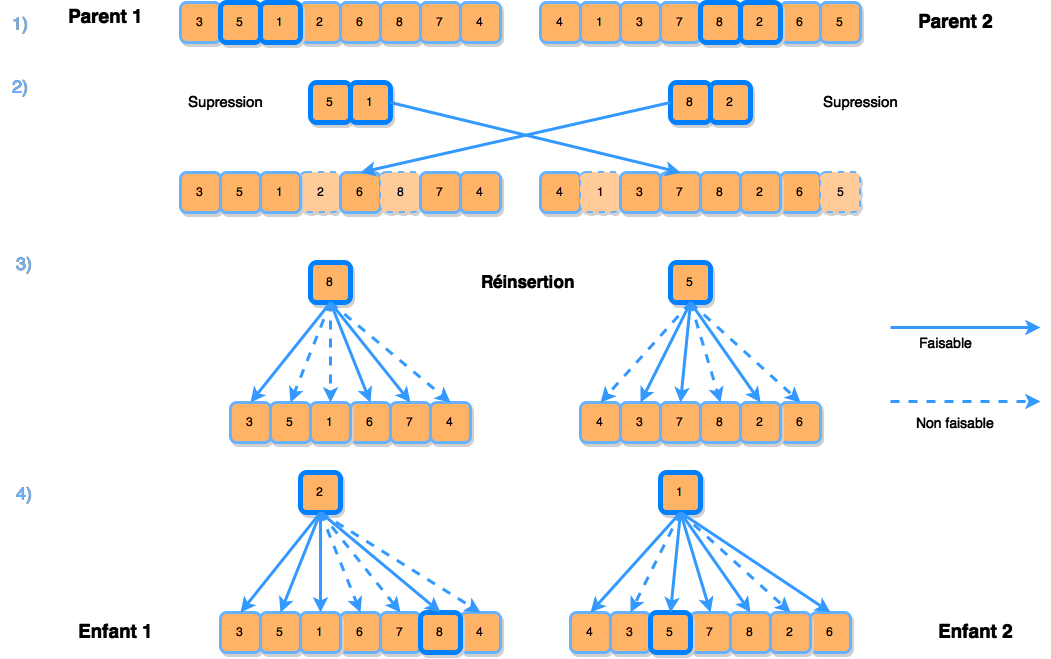
\includegraphics[width=6in]{img/BCRC.png}
		\caption{Best Cost Route Cross-over.}
	\end{center}
\end{figure}


\paragraph{Mutation} % (fold)
\label{par:Mutation}

Mutation operators provided means to randomly alter children  individual in order to improve the exploitation of the search space, where some “valley” are not accessible by any recombinaison of the current gene pool, if some gene where not in the initial population by example.
Mutation operators are domains and problems specifics, depending of the genome representation.

\paragraph{Evaluation} % (fold)
\label{par:Evaluation}
The evaluation function is the most important part of GAs, since they guide the evolutionary process to incrementally better solutions. It allows us to assign a score to the individual in regard to the problem at hand. We call that score the fitness of the individual. \\
The fitness function represents the search space and describe the fitness landscape by sampling and extrapolating it by the means of a population of individual. « Visually », the algorithm try the most intersting places of its search space (also called valley when minimizing).


\paragraph{Multi-objective selection } % (fold)

Before starting the next iteration in the generational loop, we must first selected the new « parents
» individual (surviving ones) from the set ($\lambda$ + $\mu$) of children individual $\lambda$ and parent $\mu$ of the current generation. The number of individual selected this way is equal to the original size of the parent population  $\mu$. \\
Selection procedure are based on the \emph{fitness} of individual. However, this simplistic approach were only the best (more fitted) individual are selected, i.e after sorting, yield to premature convergence.


\bigskip
During the selection process, it is necessary to keep  
Lors du processus de sélection, il est nécessaire de garder des ``good enough\cite{sharma2010archived,deb2002fast}'' individual which help maintening some sort of diversity in the global population, to the contrary of deterministic methods. \\
The best selection mecanism are in the most part stochastic like the common but efficient tournament selection, selecting the best individual from a random set of n elements. 
There are much difference when dealing with multi-objective optimimization(\emph{MOEA\footnote{Multi Objective Evolutionary Algorithm}}). The core concepts will be discussed below.



\paragraph{Optimisation
multiobjectif}\label{optimisation-multiobjectif}
The main interest of using genetic algorithm instead of other meta-heuristics come from the fact that obtained results exhibit creativity and are competitive with human intelligence. Once a certain number of generation is reached and even with randomly initialized solution, we are able to obtains "good" results. We can only defined them as "good" solution as we have no way to know when the global optimum is reached or if the optimization did get stuck in a local optimum. Traditionally we try to optimize only one criteria (objective), but it is also possible to have several at the same time even antagonistic one. The principal obstacle encountered when doing multiobjectives optimisation is the selection procedure.\\
When dealing with single objective optimization, the selection is relatively simple: the individuals taken from multiple tournaments. In the context of MOEA, how can we define "good" solution ? Is an individual fully satisfying one criteria better than one mildly satifying all ? The principle between all multi-objective selection operator (\emph{NSGA-II\cite{deb2002fast}, ASREA\cite{sharma2010archived,sharma2010gpgpu}, SPEA}) come from world of economy. It is called \emph{Pareto's optimatity} or \emph{Pareto's dominance.}

\paragraph{Pareto's dominance}\label{dominance-de-pareto}

To Pareto dominate means that for one given solution there are no other solution which have at least one criteria better than his. For \emph{MOEA}, a solution dominate an other if and only if those two condition are satisfied:


Dominer au sens de Pareto\cite{voorneveld2003characterization}, pour un élément donné, signifie qu'aucun
autre élément n'a au moins un critère meilleur que les siens. Dans le
cadre des \emph{MOEA}, une solution domine une autre si les deux
conditions suivantes sont remplies:

\begin{itemize}
\item
  Solution x1 has no fitness worse than one of solution x1
\item
  Solution x1 has at least one fitness better than one of solution x2

\end{itemize}

\begin{figure}[htbp]
	\begin{center}
		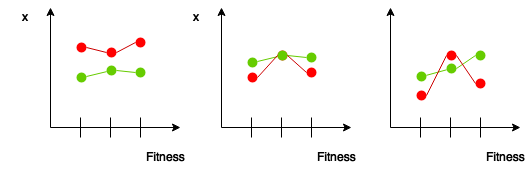
\includegraphics[width=4in]{img/paretoDominance.png}
		\caption{Thus two solution, red and green. When minimizing, from left to right, we get : green dominate red, red dominate green and neither green nor red dominate each other.}
	\end{center}
\end{figure}


% Plus formellement: // formule en laTex

From this definition, we can deduct the concept of \emph{Pareto's Front}: the set of non-dominated solutions. Pareto's front allow us to find good compromise between different criteria's profile. To define a Pareto's front is analogeous to find the convex hull\cite{godfrey2007algorithms} in a \textit{n}-dimension space, given \textit{n} the number of objective.

\label{par:Multi-objective selection }


\section{Local searches}
By design genetic algorithm provide good exploration of the search space, meaning that they sample the fitness landscape in a coarse-grain fashion.
The mutation operator setup in the evolutionary loop, provide the smaller step of the sampling also called "exploitation". The main difficulty when trying to 
solve a problem using stochastic methods or using machine learning is to have a good ratio between exploitation and exploration. This is often referred in the literature as the exploitation/exploration problem. If the exploitation is too high, the search will be quickly stuck in local optimum and if the exploration is too high the search will not converge to any useful result. \\
With the exception of the mutation operators described before, the first part of this thesis was focused in the exploration part of the algorithm, implemented last year. In this section we will describe the work done on creating and adapting popular local search methods in VRP and travelling salesman problem to our specific problem as combinatory optimization often require to be help with a set of local search algorithm, small heuristics and brute force methods.

\subsection{2-opt* for pickup-delivery}
The 2-opt* local search consist of exchanging two nodes form two different routes. If the newly defined routes
produced a better global solution as defined by the evaluation function (in the basic formulation of TSP
the new solution produced a shorter global solution in distance) ??MISSING END OF SENTENCE??


\subsubsection{Base algorithm}
To avoid unnecessary computation the algorithm uses the concept of triangular irregularity
between the old and new edges after reorganization. By doing this, there is no need to
evaluate the whole solution after each swapping, only the locally changed resulting edge.\\
\\
The whole algorithm work as follow:\\
For each node of a route, we try to swap with all the nodes of all other route and we
select the best one as defined by the evaluation function. If an improvement over the global
fitness occurred (a swap was selected) then set an improvement boolean at true.\\
\\
We continue doing the same procedure between all the nodes of the problem, resulting in a
complexity of O(n2). This local search, while exhaustive is greedy by nature and is not proved
to find the best global reorganisation of nodes, which is the task of the evolutionary loop.\\
\\
Here the formulation of the algorithm.
\begin{figure}[htbp]
	\begin{center}
		\includegraphics[width=4in]{img/2-opt.png}
		\caption{Best Cost Route Cross-over.}
	\end{center}
\end{figure}
\subsubsection{2-opt*}
The 2-opt algorithm is not adapted to time-windows variant of the TSP/VRP problem like ours.
In order to work well with the time constraint a variant of the 2-opt algorithm was developed,
called 2-opt*. A new condition must be satisfied when swapping edge. The nodes preceding and
following the selected one must verify the partial order of the time-windows, greatly reducing
the number of possible swap.\\
\\
The reformulation of the algorithm is the following:
\begin{figure}[htbp]
	\begin{center}
		\includegraphics[width=4in]{img/2-opt-star.png}
		\caption{Best Cost Route Cross-over.}
	\end{center}
\end{figure}
\subsubsection{PD-flavored version}
Unfortunately there was no variant for the pickup-delivery variant of the TSP/VRP problem.\\
We decided to extend the 2-opt* local search for PD by following the same framework used to
pass from the 2-opt to 2-opt*. In this case the new condition to satisfy before swapping is
the following: we swap the pickup and the delivery node of a journey simultaneously against the
pickup or the delivery of the selected node, while satisfying the requirements of the 2-opt*
algorithm for the two swapped node. This further reduced the possible number of swaps but only
produces legal solution.\\
\\
The reformulation of the algorithm is the following:
\\
\begin{figure}[htbp]
	\begin{center}
		\includegraphics[width=4in]{img/2-opt-star-pd.png}
		\caption{Best Cost Route Cross-over.}
	\end{center}
\end{figure}

\subsection{Intra route}
The basis of this heuristic picks two routes randomly and swaps two nodes from each route.
Without modification this really simple heuristic will not often produce legal solution in
the project context. We extended it by all swapping the other node of the journey with each other.\\
This is more a mutation than an heuristic as no score are recomputed in any way. The time-windows conditions
don't need to by satisfied because the whole individual will be sorted following the partial order operator
for time-windows before the evaluation phase.\\
\begin{figure}[htbp]
	\begin{center}
		\includegraphics[width=6in]{img/intra.png}
		\caption{Best Cost Route Cross-over.}
	\end{center}
\end{figure}

\subsection{RAR}
An other mutation-like operator implemented the Remove and Reinsert one. It consists of selecting randomly one node
in a route and inserting it back to another one. Like the others, a small adaptation was necessary.
We also remove and reinsert the sister element of the selected node. This operator is a mean
to increase the solution diversity efficiently. Contrarily to the actual algorithm, no feasibility checks are
done because they will occur during the evolutionary loop, in particular the crossover and
the evaluation phase, coming right after all local searches. \\

\begin{figure}[htbp]
	\begin{center}
		\includegraphics[width=6in]{img/rar.png}
		\caption{Best Cost Route Cross-over.}
	\end{center}
\end{figure}

\subsection{Spliting and merging}
Route splitting and merging follow the same logic of the Remove and Reinsert operator.\\
Instead of a single node it does operate on whole section of the route. A whole section
is removes from the original route to be reinserted to another one. Splitting and Merging are
dual operations in the mathematical sense of the term.\\
The differences are the following:
\begin{itemize}
  \item When splitting, the section is reinserted to an empty vehicle.
  \item When merging the section is integrated to a non-empty vehicle.
  \item Merging tries to preserve the order of the subsection but abide the time-windows partial order.
\end{itemize}
This mutation was developed because of the need to reinstate empty vehicle when optimising without
resource minimization in mind and thus is not useful when minimizing it.

\begin{figure}[htbp]
\centering
	\begin{subfigure}{.5\textwidth}
                        \centering
			\includegraphics[width=2.7in]{img/merge.png}
			\caption{Best Cost Route Cross-over.}
	
	\end{subfigure}%
	\begin{subfigure}{.5\textwidth}
                        \centering
			\includegraphics[width=2.7in]{img/merge-simple.png}
			\caption{Best Cost Route Cross-over.}

	\end{subfigure}
\end{figure}


\subsection{Fuzzing}
The fuzzing mechanism is one of the most important work done concerning the quality and concrete use
of the algorithm as it reproduces part of the methodology used by the human operator. By design the algorithm
avoids breaking all order accordingly with the partial order on the time-windows.\\
In real planning, the
appointments are taken sometimes weeks before they actually happen, often with limited vision of the future
planning for the days. With restricted resources, big delay or hard constraints can remain unsatisfied if
the problem is optimised head-on. For instance, if only three ambulances are provided and four journeys for ambulances
start at the exact same time given that ambulance in all possible configurations can only carry one passenger
 (equivalent of taking one journey) at a time, the following case will occur:
\begin{itemize}
  \item A concurrent journey with ambulance, breaking the load hard constraint on ambulance
  \item The supplementary ambulance journey will be assigned to an other type of vehicle,
        breaking the hard constraint on the assignment by vehicle type
\end{itemize}
Such result are not valid and will be unusable on the ground.\\
In some configuration taking care of a journey after another, even if it means breaking the
imposed partial ordering, will result in tremendous loss of delay. In reality, when the operator
successfully detects such problem, he's given the right to call back the client and change the
time of the appointment. \\
\\
From this problem of non optimizable journey and trivial improvement, a need naturally arises of handling
all edges cases automatically. For this purpose we decided to implement a random perturbation around the
actual time of each pickup and delivery. By adding a Gaussian distributed noise, the sorting shift around
element, allowing the possibility to the algorithm to work past its previous limitation.\\
The noise is modeled as a gene and is modified as such by the different genetic operators.
We modify our evaluation method to compute the difference between the shifted and non-shifted time
to correctly assert its benefice. Allowing the algorithm to think outside its own limitation does
have a drawback: it increases in a drastic and exponential manner the number of configurations,
what is only bound by the convergence of the evolutionary process.\\
Graph

\section{Result}
\subsection{Metrics definitions}
For further assessing the quality of the result without cluttering and losing sight of the logistic feasibility of the solution, we defined a set of metrics that in some cases is redundant with the fitness computation. \\
The goal of those metrics is to quickly and efficiently compare planning in a coarse-grained fashion. They also allow the operator to rapidly identify exploitable planning.\\
Those are actually showed in the algorithm interface. They consist of: 
\begin{itemize}
  \item The total cumulated minutes of delay
  \item The total cumulated minutes of anticipated employee starting time
  \item The total cumulated kilometers of travel without load
  \item The number of concurrent journeys
  \item The number of hard constraints violated
\end{itemize}
To also give an idea of the state of the evolution, we decided to only plot the delay
fitness allowing the operator to know when convergence has occurred.
Screenshot of the interface
\subsection{G-ASREA vs NSGAII}
\subsubsection{Sélection et ranking : NSGAII et
	ASREA}\label{suxe9lection-et-ranking-nsgaii-et-asrea}

One of the main selling point of our implementation, in order to get tremendous speed-up, is having replaced the selection algorithm \emph{NSGA-II\cite{deb2002fast}} with \emph{ASREA\cite{sharma2010archived,tsutsui2013massively}}.\\

\emph{NSGA-II} is the de facto \emph{ranking} and selection algorithm of \emph{MOEA}, withe an asymptotique complexity of O(\emph{mn\^{}2}) given \emph{m} the number of objectives and \emph{n} the number of individual.
There exist several implementation in \emph{C/C++} of \emph{NSGA-II}, which is why it was used at first as decided by  Mr. Catania.\\

With population count going higher and higher  (\textgreater{}10 000
individuals), the execution time taken by \textit{NSGA-II} become a considerable part of the total execution time,
The main idea behind \textit{NSGA-II} is to get a ordering of rank using the principe of \textit{Pareto dominance} already explained before. I then decide to use \textit{ASREA}, a recent and innovative archive-based ranking algorithm with a complexity in O (\emph{man}) given \emph{a} size of the archive, \emph{m} the number of objectives and \emph{n} the number of individual and its paralellized variant on \emph{GPGPU} , \emph{G-ASREA\cite{sharma2010gpgpu}}.

\bigskip
\emph{NSGA,} like \emph{ASREA}, are elitist selection algorithm, the first one by its deterministic ranking and the other by relying on an archive of best previous individual . A more detailed explaination of the two algorithm is available in the annexe. \\ 
The speed-up of \emph{ASREA} against \emph{G-ASREA} are quite high, up to two order of magnitude above. 
\begin{figure}[htbp]
	\begin{center}
		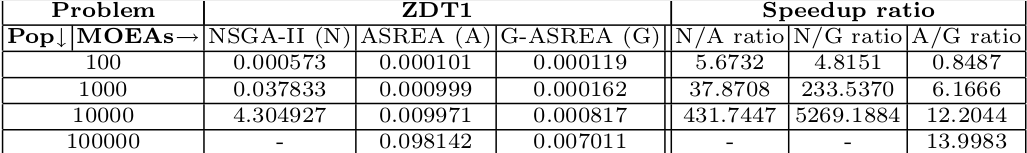
\includegraphics[width=6in]{img/asrea_table.png}
		\caption{Comparing times et speed-up between ASREA, NSGA-II and G-ASREA on a minimization of ZDT function\cite{zitzler2000comparison}.}
	\end{center}
\end{figure}

Mr. Collet gave me a base implementation of \emph{ASREA} on \textit{GPU}. The algorithm code was strongly coupled with a synthetic benchmarking program of (\emph{ZDT functions\cite{zitzler2000comparison}}).

We continued our work of paralelisation of \textit{G-ASREA}, to be able to run the integrality of the ranking inside the scope of a \textit{GPU}. After extraction, refactor and heavy adaption, we could get the following 


\begin{center}
	\begin{tabular}{ |l| c| r| }
		\hline
		Nombre d'individus & NSGA-II & G-ASREA \\
		\hline
		1024 & 5 ms & 2 ms \\
		16 384 & 464 ms & 19 ms\\
		32 768  & 1563 ms& 27 ms\\
		\hline
	\end{tabular}
	\captionof{table}{Temps de la sélection, moyennes sur 50 générations.}
\end{center}

\subsubsection{Execution time}
The main selling point of ASREA is its relatively low complexity O(man), one degree below that of a NSGA O(n2).
This permits much higher size of population resulting in a increase of diversity. By having a high diversity
among individual, the optimization is much better at avoiding local optimum and lessens the risk of premature
convergence. NSGA-II is a purely sequential algorithm and with high population count, represents as much as
99,9\% of the execution time. Here is the speed-up of our implementation of ASREA over NSGA-II. \\
The results pretty much speak for themselves, we were able to get almost 200 times faster generation
than NSGA-II. Exhaustive benchmarking are provided in the table below.
 
\subsubsection{Quality of results}
An interesting byproduct of ASREA selection is the much better solution at a given generation while converging
in a much later stage of the evolution. This is due to the high diversity and the resilience to random mutation
guaranteed by ASREA. Unfortunately we had no time for a deeper analysis of this behaviour. Here are the plots of
each fitness of the best solution at every generation of a run using ASREA against one using NSGA-II

\subsection{Comparison against human operators}
The direct comparison of planning done by human operators against the one generated by the algorithm is difficult
to survey directly. While human operators have difficulties visualizing the planning global order, that is the routing
itself, they are also the one knowing about their company specificity and all the edge cases not covered directly by
the algorithm, i.e a patient traveling only with a specific crew because of implicit reason (language, habit) or the company
not allowing or promoting certain types of configuration.\\
\\
Thus the algorithm only serves as base planning, that need to be review by a human operator in order to correct
the obvious changes of specification. However, it does all the heavy lifting in a reasonable time (less than one minute
for the whole day) with the correction taking five to ten minutes of mildly intensive work, given that by hand, the same planning
should have took one hour of intensive work. When doing planning with the help of the algorithm, one can expect a smaller
cognitive workload and saving up to 3//4 of the needed time.  

\section{Deployement and architecture}

The current version of the deployed algorithm is the CPU version. This version is in
production in a few test clients, each one having very different needs. For example,
one client does not require to do any employee optimisation and its workload is
around the high-end of what we consider small client (~200), while the other needs a
very precise and tight optimisation of their employees on small workloads (~80).\\
\\
To be able to rapidly implement different features and toggles them on depending of the client,
we developed a small middleware in Python Django to launch instance of the algorithm
with the correct set of options. The middleware also takes care of isolating the
different instances between users of the small company and serves as an orchestration
tool.\\
\\
The pipeline remains simple: the end-user configures then start the algorithm through
Saphir, Saphir then collects and exports the data to the middleware. The middleware
then starts the algorithm instances with the received data and additional options to
provide isolation.\\
\\
The GPGPU version, while being done, developed and tested, is still at the time of
writing not deployed due to the difficulty to get hardware equipped with specific
GPGPU in data centers. We wanted to avoid having to pay for a dedicated server rack
with "professional-grade" GPGPU such as Tesla K20, because our algorithm was
designed with consumer-grade graphical card such as the Nvidia 960 GTX. Using the
cloud (Amazon AWS EC2) for this project is impossible due to the high pricing
of such services.
\\
We started using Docker for easy deployment and scalability of the algorithm. Docker
is a tool for deployment, orchestration and automating, providing a layer of
abstraction and isolation over the kernel and the Linux operation system, in order
to avoid the problem related with virtual machine (slow starting time, size, etc
...). \\
Using Docker was quite informative about real-world deployment, robustness,
real-time scalability and monitoring. It is a tool that got a lot of praise those
last few year, but remains easy to use. Docker containers are light (less than 500
MB for ours), quick to deploy (a few minutes) and provide quasi-instantaneous launch
(around 300ms).

I still worked on deploying the architecture on Amazon Elastic Cloud as a back-up
solution. One of the only difficulty encountered was to get base amazon Linux image with the
correct Nvidia driver installed because it must correspond. To get a Docker
container correctly accessing the GPU, the toolkit installed on it must also
correspond with the drivers installed on the host.
The price tag of Amazon EC2 is what blocks us from using it: the optimization must
run at all time in real-time continuous mode, and the average price of GPU instance
is around 0.3 dollars per hour and per client.

\section{Role}

This year my role inside the company and the project changed quite a bit. I kept
my position as lead researcher and lead developer on the project, but I stepped
down from my position of junior project manager, due to the following reason: with
the algorithm going in production, a lot of control over the different tests and discussion with
clients, modification or implementation of features were delegated to the main
hierarchy of the company. For a more concrete example, all communications with clients now
go through the support department, before going to the main project manager of
Saphir M. Munsch and occasionally to the CTO M. Philips.\\
As the project did finally come to completion, more and more employees and fellow
developers of Synovo became familiar with the project, its goals, underlying
concepts and core functionalities. \\
I was still responsible for all decisions concerning design, implementation
and used technology for each features and requirements. There was a lot of back and
forth between me and the main beta client/user GAGN concerning their needs and
the possibility to integrate their specific business logic efficiently as it was
sometimes conceptually incompatible with evolutionary process. Such demands often
came from the need to enforce a constraint early-on the optimization, but potentially
shifting the fitness landscape to a less interesting one. It was also I that was the
architect of the future infrastructure and deployment. \\
I learned a lot about modeling development pipeline and processes and releasing a
product with everything around it: user feedback, bug tracking, support, public
documentation. I was thus able to further improve my knowledge of the professional
and corporate world. We will discuss and expand these items in the followings sections.

\subsection{Decision-making and crisis-managing}
Like enunciated before, I was the sole manager of the scientific side of the project.
It was very intellectually intensive as well as stressful, some features couldn't be
implemented directly but implicitly through subtle fitness value ranking and
scaling. Most time though, an ad-hoc approach regarding the addition of new condition
worked well. When adding condition and new "sub-fitness" to an EA, one must to guard to
avoid guiding to evolution to a unadapted fitness landscape. \\
In some cases, it was the utility of the asked features that were discussed. Some demands
did not fit at all to the general framework of evolutionary algorithm. My work in this
case consisted of finding a compromise between the client's demand and the feasibility
of such demands. It did revolved a lot around finding a subsumption of the business
rules loosely related to the feature. To be able to do this, one must have a very deep
understanding of the domain that he tries to optimize for. Some demands were just not
feasible at all (such as requiring to solve an other NP-hard sub-problem) or clearly
misguided and it was my responsibility as the Lead researcher to explain and refuse
such demands, in a clear and professional way.\\
By component of my decision-making process was time, in multiple dimension. First, the time
needed to design and implement a feature, modification or improvement, as well as
debugging it in the stricto census meaning of the term in software engineering. Secondly,
the time needed to explain the behaviour and trajectory of the evolution in case of problem.
This is difficult to estimate at all, because there are no tools for it nor methodology.
It was necessary to be able to give satisfactory explanation to client and observer,
to help them get the core ideas between GA.

\subsection{Stitching everything together}
There were some period where it was exhausting to be the one-man orchestra of the project.
To be able to fill the role it was a priority to get to know and expand some domain of
software engineering that I had not previously touched. \\
Those unknowns subject were more specifically related to the "Ops" part of the "devOps"
job: managing machines, server, monitoring production system, orchestration, logging, and so on.\\
\\
One detail that struck me a bit was that when I were not around or not focus on the job,
the project seemed to lose its momentum due to the lack of leadership. This feeling
remained until the beginning of July, with the now working and in production GPGPU
version when Synovo higher-up pushed the product from the RD department to Saphir,
effectively integrating it with the main application.


\subsection{Difficulties}
For all R\&D projects the most terrifying thing is to be lost on a problem and
having already explore the literature and the common ideas.\\
This fear and feeling come by the fact that research is a creative field and share the
problematic of all creative fields. I did experiment this situation and frustration first-hand.
When stuck, all project planning fall flat, as it is next to impossible to give correct estimation
of time needed to overcome the obstacle. This sentiment is further magnified because of traditional corporate
context with fixed hours. The lack of productivity kind of enhanced the frustration,
creating a stressful feedback loop.\\
To escape it, one must be resourceful and critical of the work already done. It does take effort discarding previously
working modules and ideas, but in fine, it is by reshuffling and reinventing the global shape of the project that:
\begin{itemize}
  \item New constraints are implemented cleanly and efficiently
  \item New ideas can be developed from the freed space following restructuring
  \item Problems can be skipped or resolved themselves implicitly
\end{itemize}
    

\section{Conclusion}

The ILC master is, at the time of writing this memoir, my best professional and personal experience.
The sheer amount of subject explored, difficulties overcame, productivity and learning, from so many
different angles make it an invaluable experience.\\
Since there is so much to cover in this concluding part, we will follow this plan: the master program and apprenticeship
itself and how it was conducted, the work and research done in both the public and private institution and their scope,
what it did make me learning from the personal standpoint, the good it provided for my future career and finally a
reflection on the importance of automating tasks in the current economic context.\\
\\

%% Super master
This type of formation is extremely important as it gives the student clear entry in the corporate world while
still providing a high-level academic education. In France, we should clearly put an emphasis on this type of education.\\
\\
%% Super experience 
I did struggle a little bit at first to get an good life/college/work balance. Once the first month went by I did find
a correct equilibrium. While those two year were clearly the richest of my life in term of productivity, it did tend to
be tiring, due the constant context switching.\\
I did have a particular status inside this master, working on two different project and research structural,
one public and academic, the ICube laboratory attached to the University of Strasbourg and one private and
startup-y, my work at Synovo as lead researcher. By having the chance to see both kind a structure it gave me an
unprecedented view and scope on the research world. For it, I am grateful to both Pr. Collet and M. Wies which make it happen.
Sometimes fully independent, sometimes project manager, it was two years of concentrated work experiences.\\
\\
%% Content  
The content of the work done was tremendously interesting. It was always my desire to work in the fields of narrow AI and
having to design and implement framework, then full genetic algorithm was the best introduction one can dream of. As stated before
it was not an easy task: a lot of effort was given to be able to get a commercial capable project. The domain of healthcare routing
was not explored at all in France due to the difficulty to extract clear, workable data and concept for EA.\\
\\
%%Personal satisfaction 
Having finally completed this big and complex project, I hold a great feeling of satisfaction.
This ends a four years collaboration between Synovo and the ICube laboratory. A lot of heart was poured in this project from
all the different participants and contractors and by having it running with GPGPU on production is a wonderful accomplishment.
From a personal perspective, having this project on my portfolio is one of the best reward a college graduate in Computer Science can get.\\
\\
%%Paradigm
This project holds a special interest, in the mist of the current economic context because in a way it goes to the direction
of the probable paradigm shift of mass automating of services and means of production. It removes painful and repetitive task
with a high level of cognitive load, enabling the human to more interesting and diverse task instead.
From the economic standpoint, it also allows the company to save money on the routing itself and on the human work required to get planning. \\
\\

\bibliographystyle{plain}
\bibliography{thesis}

\end{document}
